\begin{subfigure}[t]{0.48\linewidth}
    \centering
    \begin{tikzpicture}
        \begin{axis}[
            ybar,
            bar width=8pt,
            width=0.95\linewidth,
            height=0.23\textheight,
            ymin=0, ymax=1.05,
            symbolic x coords={Highway,City},
            xtick=data,
            ylabel={$a_{\mathrm{ord}}$},
            title={Weighted order agreement},
            title style={font=\sffamily\small\bfseries},
            label style={font=\sffamily\small},
            tick label style={font=\sffamily\scriptsize, text=black!75},
            legend style={
                font=\sffamily\tiny,
                at={(0.5,0.97)},
                anchor=north,
                legend columns=2,
                draw=black!8,
                fill=white,
                fill opacity=0.92,
                text opacity=1,
                rounded corners=2pt,
                inner xsep=3pt,
                inner ysep=2pt,
            },
            axis line style={draw=black!35},
            tick style={draw=black!35},
            grid=major,
            major grid style={draw=black!7, line width=0.25pt},
            enlarge x limits=0.28,
            nodes near coords,
            every node near coord/.append style={font=\sffamily\tiny, text=black!70, yshift=1pt},
            every axis plot/.append style={draw opacity=1},
        ]
            \addplot+[fill=black!18, draw=black!55] coordinates {
                (Highway,0.40) (City,0.90)
            };
            \addlegendentry{Base}
            \addplot+[fill=blue!60, draw=blue!70!black] coordinates {
                (Highway,0.40) (City,0.50)
            };
            \addlegendentry{Multi}
        \end{axis}
    \end{tikzpicture}
    \caption{$a_{\mathrm{ord}}$ on the reduced offline joint sweep.\label{fig:inverse_offline_metrics_a}}
\end{subfigure}\hfill
\begin{subfigure}[t]{0.48\linewidth}
    \centering
    \begin{tikzpicture}
        \begin{axis}[
            ybar,
            bar width=8pt,
            width=0.95\linewidth,
            height=0.23\textheight,
            ymin=0, ymax=1.05,
            symbolic x coords={Highway,City},
            xtick=data,
            ylabel={$r_1$},
            title={Top-priority recovery},
            title style={font=\sffamily\small\bfseries},
            label style={font=\sffamily\small},
            tick label style={font=\sffamily\scriptsize, text=black!75},
            axis line style={draw=black!35},
            tick style={draw=black!35},
            grid=major,
            major grid style={draw=black!7, line width=0.25pt},
            enlarge x limits=0.28,
            nodes near coords,
            every node near coord/.append style={font=\sffamily\tiny, text=black!70, yshift=1pt},
            every axis plot/.append style={draw opacity=1},
        ]
            \addplot+[fill=black!18, draw=black!55] coordinates {
                (Highway,0.0) (City,1.0)
            };
            \addplot+[fill=blue!60, draw=blue!70!black] coordinates {
                (Highway,0.0) (City,0.5)
            };
        \end{axis}
    \end{tikzpicture}
    \caption{$r_1$ on the same sweep.\label{fig:inverse_offline_metrics_b}}
\end{subfigure}
